\chapter{Background}
\label{cha:background}
%At the begging of each chapter, please introduce the motivation and high-level
%picture of the chapter. You also have to introduce sections in the
%chapter. 

\epigraph{People shouldn't be afraid of their government. Governments should be afraid of their people..} 
{\textit{Alan Moore, V for Vendetta }}
  Counting ballots by hand is tedious, error prone, slow, and costly process. 
  For example, the Senate election conducted in Western Australia in September 2013 was 
  declared void by the high court because of the loss of 1370 votes. It was 
  re-conducted in April 2014 at the cost of 20 Million 
  AUD with additional  delay in results \citep{Aussentate}. Before introduction to 
  electronic voting machines in India, it will take month to declare the result.
  As a consequence, many countries 
  are now adopting electronic voting to alleviate the problems introduced by hand counting. 
  
  The world can be divided into five broad categories according to 
  the usage of electronic voting \citep{Evoting} \ref{fig:world_electronic_voting_map}: i) No electronic 
  voting (Grey Area), ii)
  Discussion and/or voting technology pilots (Yellow Area), 
  iii) Discussion and concrete plans for Internet voting (Orange Area),
  iv) Ballot scanners, Electronic Voting Machines, and Internet Voting (Green and Dark Green),
  v) Withdrawn voting technology because of public concern (Red Area) 
    \begin{figure}[htb]
	\begin{center}
	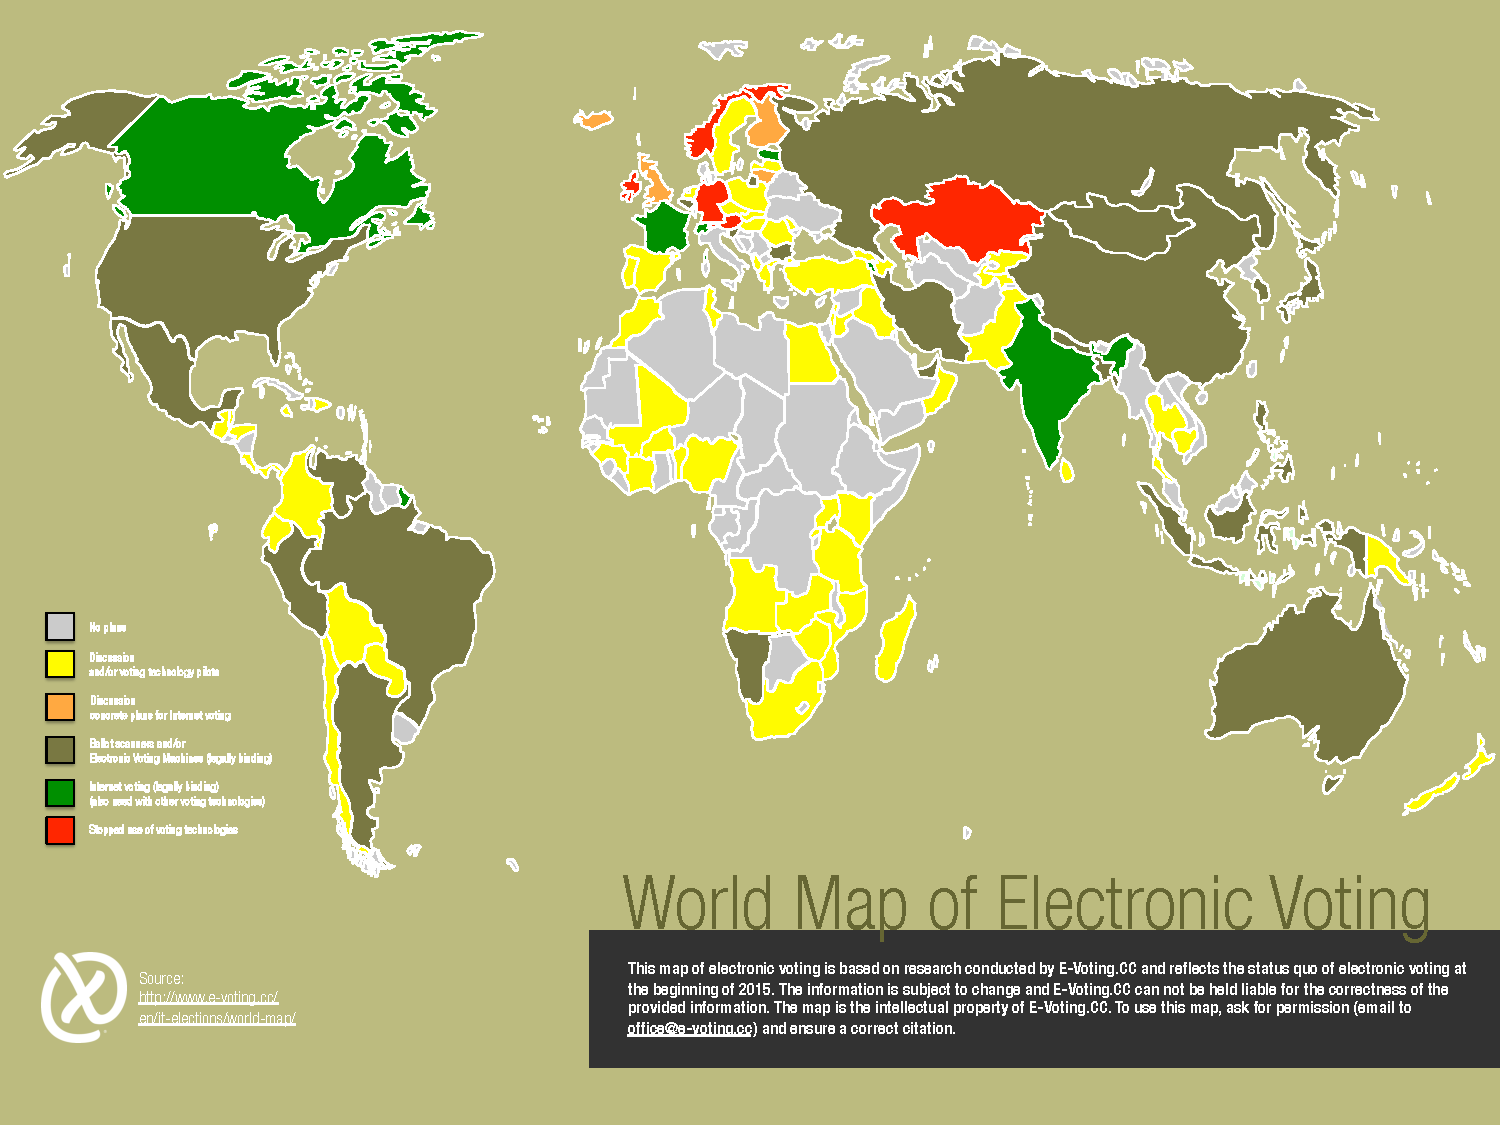
\includegraphics[scale=0.5]{e-voting_worldmap_2015.pdf}
	\caption{World map of Electronic Voting}
	\label{fig:world_electronic_voting_map}
	\end{center}
  \end{figure}  
 
 
\textbf{Chapter Outline:}
  Write here a chapter outline

\section{Electronic Voting}
  Electronic voting is projected as a step towards the future with 
  many benefits, such as increased voter turnout, faster result, 
  accessible to everyone including challenged voters, and reduced 
  carbon footprint (for each 
  national election, India saves about 10,000 tonnes of the ballot 
  paper by using electronic voting machines). 
  There is no doubt that electronic voting has many advantages 
  over paper ballot, but it is certainly not flawless.  
  Electronic voting makes 
  the process faster, but it has its own layer of added complexities 
  which creates trust issues amongst voters. For this reason, some countries 
  who were the early adopters were also the early abandoner, e.g.
  Germany, and The Netherlands (countries in red color in the world map 
  \ref{fig:world_electronic_voting_map}).
  
  
  \textbf{Germany:} In 2005 German election, two voters filed a case in the German 
  Constitutional Court (Bundesverfassungsgericht) because their 
  appeal to scrutinize the election 
  was not heeded by the Committee. They argued that using electronic 
  voting machines to conduct the election was unconstitutional. Furthermore,
  they added that
  these machines could be hacked, hence results of the 2005 election 
  could not be trusted on the grounds 
  of public examinability of elections according to German Constitution 
  (Basic Law for the Federal Republic of Germany) \citep{Germanconst}. 
  The Court noted that, under the constitution, elections are 
  required to be public in nature:\citep{Germanconst}
  
  \begin{displayquote}
  The principle of the public nature of elections requires that all 
  essential steps in the elections are subject to public examinability
  unless other constitutional interests justify an exception. 
  Particular significance attaches here to the monitoring of the 
  election act and to the ascertainment of the election result.
  \end{displayquote}
  
 
 
  \noindent	
  In its verdict, the court did not rule out or prevent the usage of electronic 
  voting machines,  but suggested to make the process more 
  transparent and trustworthy \citep{Germanconst}.  
  
  \begin{displayquote}
  The legislature is not prevented from using electronic voting machines 
  in the elections if the constitutionally required possibility of a 
  reliable correctness check is ensured. In particular, voting machines 
  are conceivable in which the votes are recorded elsewhere in addition
   to electronic storage. This is for instance possible with electronic
   voting machines which print out a visible paper report of the vote 
   cast for the respective voter, in addition to electronic recording 
   of the vote, which can be checked prior to the final ballot and is
    then collected to facilitate subsequent checking. Monitoring that is
     independent of the electronic vote record also remains possible when
     systems are deployed in which the voter marks a voting slip and the 
     election decision is recorded simultaneously, 
     or subsequently by electronic means in 
     order to evaluate these by electronic means at the end of the 
     election day.
     \end{displayquote}
  
  \textbf{The Netherlands:}
  The Netherlands was among a few countries who adopted electronic voting 
  in the early nineties (1990), but it did not go very well in the long 
  run and was abolished in 2008 \citep{Jacobs2009}. 
  The reason for abolishing the electronic voting was that   
  the voting machines used in elections were susceptible to many attacks,
  and the results of elections conducted using these machines 
  were not publicly verifiable.  Besides, a Dutch public foundation, Wij vertrouwen stemcomputers niet
  (We do not trust voting computers), demonstrated that e-voting machines 
  used in election leaks enough information to guess the choice of a voter 
  from distance of 20 to 30 meters  \footnote{https://www.youtube.com/watch?v=B05wPomCjEY}.
  
  
  
  Germany and The Netherlands are some of the rare cases where 
  electronic voting was withdrawn because it was not able to 
  replicate the same trust environment as created by paper 
  ballot systems whereas Australia, and India continued 
  with electronic voting despite having the concerns expressed 
  by researchers about the security of system. 
  
  \textbf{India:}
  India, one of the largest democracies in world, 
  uses electronic voting machines (also known as EVMs) for national 
  and state level  elections despite the fact that many political parties have raised security 
  concern against it. Moreover, it has already been shown in \citep{Wolchok:2010:SAI:1866307.1866309}  that it 
  is possible to manipulate the election results by replacing the 
  parts of machine with malicious look alike components. These components 
  were capable of receiving instruction over wireless communication. As a result, any malicious 
  attacker can control these components from nearby vicinity by sending 
  instructions over wireless channel by using a simple hand-held device and 
  can  manipulate the results in their favour \footnote{https://indiaevm.org/}.
  India is mainly criticised for keeping the design of electronic voting machines 
  a closely guard secretes. However, it is not impossible to get access of 
  these machines as shown by \citep{Wolchok:2010:SAI:1866307.1866309}. 
  The worst part, the design of these machines were never audited by 
  any independent third party. 
  
  

 \textbf{Australia:}
  In March, 2015 state election 
  of New South Wales, Australia, a Internet voting system, iVote,    
  was used and 280,000 votes were cast through it. NSW Election 
  commissioner claimed that it was:
  
  \begin{displayquote} 
  It's fully encrypted and safeguarded, it can't be tampered with, 
 and for the first time people can actually after they've voted 
 go into the system and check to see how they voted just to make 
 sure everything was as they intended \citep{NSWelection}.
 \end{displayquote}
 

  \noindent
  The voting on iVote 
  opened on Monday March 16 and continued until March 28. On 22 March,
  two security researchers, Vanessa Teague and J. Alex Halderman, 
  announced that iVote has critical security bug, and they demonstrated 
  that it was good enough to steal any ballot. From their paper
  \citep{10.1007/978-3-319-22270-7_3}:
  
  \begin{displayquote}
  
  
   While the election was going on, we performed an independent,
   uninvited security analysis of public portions of the iVote 
   system. We discovered critical security flaws that would allow
   a network-based attacker to perform downgrade-to-export 
   attacks, defeat TLS, and inject malicious code 
   into browsers during voting. We showed that an attacker could
   exploit these flaws to violate ballot privacy and steal votes. 
   We also identified several methods by which an attacker could
   defeat the verification mechanisms built into the iVote design.
   
   \end{displayquote}
  
  \noindent
  Basically New South Wales ran a online election for 6 days on 
  buggy software which was susceptible to many attacks with a possible 
  outcome of tampered ballot without anyone noticing it. 


   There are various factors for these debacles, but one of the most 
   common denominator among all these debacles,
   which contributed significantly,  is the software/hardware used in the election process 
   were buggy. Furthermore, these software 
   are closely guarded secrets and their source 
   code in not open for general public because of commercial 
   interests of companies \citep{AEC:2013:LMM} involved in the 
   process.
   In general, no entity related to government or electoral commission develops the electronic 
   voting software, and predominantly it is outsourced 
   to companies having experience in electronic voting software development.  
   The process 
   of turning a vague idea into a 
   concrete software, also known as software development process, involves 
   requirement gathering, software design, implementation, testing, and maintenance. 
   During this whole process of software development, software testing is the only 
   mechanism for quality assurance. However, testing is not enough for 
   instilling the confidence in software that it is bug free 
   as stated by Edsger W. Dijkstra \citep{Dijkstra:1972:HP:355604.361591}:
   \begin{displayquote}
   Program testing can be used to show the presence of bugs, 
    but never to show their absence!
   \end{displayquote}
   Additionally, most of these companies have poor testing practices which 
   exacerbate the software quality problem.
   
   In the next section, given the mission critical importance of electronic voting software 
   I will discuss that software testing 
   in not sufficient for these software, and we should 
   prove the  correctness of these software
   by using formal verification techniques \citep{BECKERT2014115}.
   Furthermore, I will argue that  having a formal verification software development methodology would alleviate 
	the bug problem with few case studies as a supporting evidence. The success of these 
	case studies should be a good motivation for us to 
	adopt formal method for electronic voting software development. 
   
   
   \subsection{Correctness: Formal Method Approach}

%	\fix {Write here the software bug story and how they could have 
%	been avoided by formal verification. Pave the path to 
%	next part of Estonia}     
%	
%	
%	One of the biggest reason for having a little or no trust at all 
%	in electronic voting is a mere possibility of bugs in 
%	the deployed software could lead to incorrect result.  
%	In this section, I will argue that 
%	having a rigorous software development methodology would alleviate 
%	the bug problem with few case studies. The success of these 
%	case studies would be good enough motivation, I hope, for us to 
%	adopt their approach for electronic voting software development. 
%    [Add a emphasis here that there is no silver bullet, but 
%     innovations attacking essential complexity could lead to
%     significant improvements. Fred Brooks 
%     There  is  no magic bullet technique that solves all the 
%     problems, but a coordinated  application  of  a  
%     range  of  techniques  does work.] 	

  
	
%	\subsubsection{Common Criteria Software Certification}    	
%	[software certification]
%	EAL 1 : Functionally Tested 
%	EAL 7 : Formally Verified Design and Tested
%	but it leaves the gap between Design and implementation.
%	Write something good about it, but this is not rigorous because 
%	it leaves the gap between design and implementation ? 
%	https://ts.data61.csiro.au/projects/TS/l4.verified/numbers.pml	
%	MicroSoft NT kernel was EAL4 certified, but it was full of bugs, 
%	so it's certainly not the approach we should take for electronic 
%	voting.		    
		    
%	\subsubsection{Formally Verified Software}
	Formal verification has been successfully applied in many areas ranging 
	from verified C compilers CompCert \citep{DBLP:conf/popl/Leroy06}, verified ML compiler
	CakeML \citep{Kumar:2014:CVI}, Vellvm: Verifying the LLVM 
	\citep{10.1007/978-3-642-35308-6_6}, verified cryptography 
	Fiat-crypto \citep{DBLP:conf/sp/ErbsenPGSC19}, verified 
	operating system CertiKOS \citep{DBLP:conf/apsys/GuVFSC11} and 
	SeL4 \citep{DBLP:conf/sosp/KleinEHACDEEKNSTW09}, verified theorem 
	prover Milwa \citep{DBLP:conf/itp/MyreenD14}, 
	verified crash resistant file system FSCQ \citep{Chen:2015:UCH:2815400.2815402}, 
	verified distributed system 
	Verdi \citep{DBLP:conf/pldi/WilcoxWPTWEA15} , mechanisation of 
	Four Color Theorem \citep{10.1007/978-3-540-87827-8_28}, 
	Fundamental Theorem of 
	Algebra \citep{10.1007/3-540-45842-5_7}, and Kepler Conjecture \citep{hales-kepler}.
	One thing I would like to emphasize 
	is that none of these are toy project, and it takes years 
	to develop and verify them. Also, some of these products 
	are used commercially e.g CompCert is used by AIRBUS, and MTU
	\footnote{https://www.absint.com/compcert/} and Fiat-crypto is used 
	in Google's BoringSSL library for elliptic-curve arithmetic 
	\footnote{https://deepspec.org/entry/Project/Cryptography}. 
	The very basic question to ponder about using formal method to develop 
	software:  does it achieve the goal, produces bug free software,  
	given the cost and effort?
	
	I would give two anecdote to answer this question. 
	One of the most basic way to 
	break the software is generating random tests and throwing it to 
	the software under consideration \citep{Miller:1990:ESR:96267.96279}.
	\citep{Yang:2011:FUB:1993316.1993532} developed random 
	C program generator and used these programs to test various 
	compilers. In three years of its usage, they have found 325 unknown
	bugs in various compiler including GCC
	\footnote{https://embed.cs.utah.edu/csmith/gcc-bugs.html} and LLVM
	\footnote{https://embed.cs.utah.edu/csmith/llvm-bugs.html}; however, 
	they could not find any bug in verified component of CompCert. 
	In their own words \citep{Yang:2011:FUB:1993316.1993532}:
	
	\begin{displayquote}
	
	The striking thing about our CompCert results is that the middle-end 
	bugs we found in all other compilers are absent. As of early 2011,
	the under-development version of CompCert is the only compiler we
	have tested for which Csmith cannot find wrong-code errors. This is
	not for lack of trying: we have devoted about six CPU-years to the
	task. The apparent unbreakability of CompCert supports a strong
	argument that developing compiler optimizations within a proof
	framework, where safety checks are explicit and machine-checked,
	has tangible benefits for compiler users.
	
	\end{displayquote}
	
	\noindent
	Formal verification is not only helpful in proving the correctness, 
	but sometimes, it helps in uncovering the bugs in design of
	software. ACL2, a Lisp based theorem prover, helped 
	AMD to uncover a floating point bug in Athelon processor which 
	has survived 80 million floating point test cases! 
	In the paper, Milestones from the Pure Lisp theorem prover to ACL2
	\citep{Moore2019}, Moore, one of the developer of ACL2, writes:
	
	\begin{displayquote}
	
	When AMD developed their translator 
	from their register-transfer language (in which designs
	are expressed) to ACL2 functions they ran 80 million 
	floating point test cases through the ACL2 model of 
	Athlon’s FMUL and their own RTL simulator. However, the 
	subsequent proof attempt exposed bugs not covered by the
	test suite. These bugs were fixed before the Athlon was 
	fabricated.
	
	\end{displayquote}
  
   \noindent
   There are numerous instances where formal verification 
	was very useful, and it caught the lurking bugs in design in early 
	stage which could never have been found by testing.
	
	For electronic voting software used in democratic election, where we 
	can not afford to lose a single ballot or miscalculation 
	or any undefined behaviour, should be developed 
	using formal method techniques.
	In order to ascertain that the formal verification of voting software has been 
	carried out diligently, one therefore needs to
	\begin{enumerate}
	\item read, understand and validate the formal specification: is it 
	error free, and does it indeed reflect the intended functionality?
	\item scrutinize the formal correctness proof: has the verification
	been carried out with due diligence, is the proof complete or does
	it rely on other assumptions?

	\end{enumerate}			
	
	\noindent
	The above mentioned requirements can be met by publishing or open sourcing
	both the
	specification and the correctness proof so that the specification
	can be analysed, and the proof can be replayed (inside the tool used for 
	verification) by any independent third party. Both need a
	considerable amount of expertise, but it can be carried out by (ideally
	more than one group of) domain experts.
	

	
	  
	 
		
 \subsection{Verifiability: Trust in Electronic Voting}
  Formal verification is useful in producing the 
   bug free code, but we solely can not 
   establish the trust in the system based on argument of 
   formal verification. The reason is that how would a voter
   \begin{itemize}
   \item ascertain that it was indeed the verified program that was
	executed in order to obtain the claimed results?
	
   \item ensure that the computing equipment on which the (verified)
	program is executed has not been tampered with or is otherwise
	compromised?
	
   \end{itemize}
   
   \noindent
   Formal verification is certainly a necessary thing in electronic voting because 
   it helps in achieving the correctness of software, but it is not sufficient because
   it has no mechanism to provide  verifiability.
   Combing both \emph{verification} of the
	computer software that counts votes, and
	\emph{verifiability} of individual counts are critical for
	building trust in an election process. These two facts, 
	 \emph{verification}  and \emph{verifiability}, 
	 can also be viewed as 
    two sides of a coin from the perspective of two major stake holders of 
    a democracy: i) electoral commission/government, and, ii) voters/participants.  
    Using formally 
    verified software to count the ballots would increase the confidence 
    of electoral commission that he has announced and published the correct result, and 
    the published result always verifies would increase the confidence
    of voter in the system. 
	 
	 
	Given the mission-critical importance of
	 correctness of vote-counting,
	both for the legal integrity of the process and for
	building public trust,  it is crucial to replace the
	currently used black-box software for vote-counting with a
	counterpart that is both verified and produces 
	evidence which can later be used to certify
	the outcome of election \citep{Bernhard:2017:PES} \citep{Rivest:2008:PTRS}.
	
	
        
%    Correctness and verifiability of electronic voting software can also be viewed as 
%    two sides of a coin from the perspective of two major stake holders of 
%    a democracy: i) electoral commission/government, and, ii) voters/participants.  
%    Using formally 
%    verified software to conduct the election would increase the confidence 
%    of electoral commission that he has produce the correct result, and 
%    the produced result always verifies would increase the confidence
%    of voter in the system. 
    
    
   
	
	
%In order to ascertain that the results of a verified program are
%indeed correct, one therefore needs to
%\begin{enumerate}
%\item read, understand and validate the formal specification: is it
%error free, and does it indeed reflect the intended functionality?
%\item scrutinize the formal correctness proof: has the verification
%been carried out with due diligence, is the proof complete or does
%it rely on other assumptions?
%\item ensure that the computing equipment on which the (verified)
%program is executed has not been tampered with or is otherwise
%compromised, and finally
%\item ascertain that it was indeed the verified program that was
%executed in order to obtain the claimed results.
%\end{enumerate}
%
%\noindent
%The trust in correctness of any result rests on all items above.
%The second two items are
%more problematic as they require trust in the integrity of
%equipment, and individuals, both of which can be hard to ascertain
%once the computation has completed. The
%first two trust requirements can be met by publishing both the
%specification and the correctness proof so that the specification
%can be analysed, and the proof can be replayed. Both need a
%considerable amount of expertise but can be carried out by (ideally
%more than one group of) domain experts. Trust in the correctness of the
%result can still be achieved if a large enough number of domain
%experts manage to replicate the computation, using equipment they
%know is not compromised, and running the program they know has been
%verified. As such, trust in \emph{verified} computation mainly rests
%on a relatively small number of domain experts.
   
   
   
\subsection{Aspects of Verification and Verifiability}
Any system for counting votes in democratic elections needs to
satisfy at least three conditions: (1) each person's vote must be
counted accurately, according to a mandated procedure, (2) the
system and process should be subjectively trusted by the electorate,
(3) there should be an objective basis for such trust, or in other
words the system must be trustworthy. While subjective trust cannot
be guaranteed through greater transparency \citep{ONeill:2002:QT}, transparency about
both the voting system and the actual counting of the vote in a
particular election are important in reducing errors and ensuring an
accurate count, promoting public trust and providing the evidential
basis for demonstrated trustworthiness. In particular, it is a lack
of transparency that has been the primary source of criticism of
existing systems, both in the literature
\citep{Carrier:2012:VCT,Conway:2017:ANS} and among civil
society organisations \citep{Vogl:2012:WWC} (for example,
\texttt{blackboxvoting.org} and
\texttt{trustvote.org}). International commitment to transparency is also
demonstrated through initiatives such as the Open Government
Partnership. Another important concept referred to both in the
literature and by civil society organisations is public
accountability, which requires both giving an “account” or
explanation to the public and when called on (for example, in court)
as well as being held publicly responsible for failures.
Transparency is thus a crucial component of accountability, although
the latter will involve other features (such as enforcement
mechanisms) that are beyond the scope of this paper. 

There are two contexts in which transparency is important in the
running of elections. First, there should be transparency in Hood's
sense \citep{Hood:2001:T} as to the process used in elections generally. This is
generally done through legislation with detailed provisions
specifying such matters as the voting method to be used 
%(as noted above, the Schulz method is not generally used in public office
%elections)
 as well as the requirements for a vote to count as valid.
In a semi-automated process, this requires a combination of
legislation (instructions to humans) and computer code (instructions
to machines). The second kind of transparency, corresponding to
Meijer’s use of the term \citep{Meijer:2014:T}, is required in relation to the
performance of these procedures in a specific election. In a manual
process, procedural transparency is generally only to
intermediaries, the scrutineers, who are able to observe the
handling and tallying of ballot papers in order to monitor officials
in the performance of their tasks. While the use of a limited number
of intermediaries is not ideal, measures such as allowing
scrutineers to be selected by candidates (eg Commonwealth Electoral
Act 1918 (Australia) s 264) promote public confidence that the
procedure as a whole is unbiased. However imperfect, procedural
transparency reduces the risk of error and fraud in execution of the
mandated procedure and enhances trust. 

Electronic vote counting ought to achieve at least a similar level
of transparency along both dimensions as manual systems in order to
promote equivalent levels of trust. Ideally, it would go further
given physical limitations (such as the number of scrutineers
able to fit in a room) apply to a smaller part of the process. The
use of a verified, and fully verifiable system is transparent in both senses, with members of
the public able to monitor both the rules that are followed
and the workings and performance of the system in a particular
instance. 

First, the vote counting procedure needs to be transparent. For
electronic vote counting, the procedure is specified in both
legislation (which authorises the electronic vote counting
procedure) and in the software employed. The use of open source code
ensures that the public has the same level of access to instructions
given to the computer as it has to legislative commands given to
election officials. The use of open source code is crucial as is
demonstrated through a comparison of different jurisdictions of
Australia. In Australia, for example, the Federal Senate and NSW
state election vote counting are based on proprietary black box
systems while the Australian Capital Territory uses open source
eVACS software
\citep{AEC:2013:LMM,Conway:2017:ANS,EA:2016:EVC}. This has
significant impact on the ability of researchers to detect errors
both in advance of elections and in time to correct results
\citep{Conway:2017:ANS}.
Private verification systems have been less successful, in both
Australia and the US, in providing equivalent protection against
error to open source software
\citep{Carrier:2012:VCT,Conway:2017:ANS}. Further, private
verification provides a lower level of public transparency than the
use of manual systems which rely on public legislation (instructions
to humans) as the primary source of vote counting procedures
\citep{Carrier:2012:VCT}. It
should also be noted that there are few public advantages in secrecy
since security is usually enhanced by adopting an open approach
(unless high quality open source vote counting software were
unavailable), and private profit advantages are outweighed by the
importance of trust in democratic elections. 

Second, verifiability provides a method of ascertaining the
correctness of
results of a specific election. External parties are able to check a
certificate to confirm that the counting process has operated
according to the rules of the voting procedure.
% (here, the Schultz method). 
Under a manual process, tallying and counting can only be confirmed by a small number of scrutineers directly observing human
officials. The certification process allows greater transparency not
limited to the number of people able to fit within a physical space,
although we recognise that physical scrutiny is still required for
earlier elements of the voting and vote counting process (up to
verification of optical scanning of ballots). Certification reduces
the risk of error and fraud that would compromise accuracy and
provides an evidence-base for trustworthiness. It is also likely to
increase subjective public trust, although this will require
engagement with the public as to the nature of verification
involved. While it is likely that in practice checking will be
limited to a small group with the technical expertise,
infrastructure and political interest to pursue it, knowledge as to
the openness of the model is likely to increase public trust.
Currently in Australia, neither open source nor proprietary vote
counting systems provide an equivalent level of procedural
transparency for monitoring the count in a particular election (for
example, compare Commonwealth Electoral Act 1918 (Australia) s
273A). 

Ultimately, legislation, computer code (where relevant) and
electoral procedures need to combine to safeguard an accurate count
in which the public has justified confidence. The verification and
verifiability measures suggested here go further to ensure this than
current methods used in Australia and, as far as we are aware,
public office elections around the world.


   		
		
   
%   \subsection{Estonia : Success Story}
%   \fix{Write the details which made Estonia a success story}
%	Estonia Internet voting is far from being perfect, but so far 
%	it has sustained all the attempts to hack it. So what made 
%	Estonian system successful despite the obvious problems. 
%	They always keep their software updated [Read more on it and
%	write a nice narrative]
	

  
    
%    Write here about Trust is highly dependent on Culture. How
%    corruption affects it and how do we perceive trust.    
%   
%   	
%    
%    In Germany and The Netherlands, paper ballot is trusted more, 
%    while Nigeria trusts more in electronic voting. 
%    
%	In paper ballot election, voters assumes that once he cast his
%	ballot and put it in to ballot box and once it reached to counting 
%	booth then his ballot will be included in count. 
%	Every party appoints his own team of scrutineers to observe 
%	the counting, so trust here is not assumed, but enforced. 
%		
%	  
%      What is the meaning of trust in electronic voting. 
%       It should allow voters and election observers to verify, 
%       independently of the hardware and software running the 
%       election, that votes have been recorded, tallied and 
%       declared correctly.
%       
%       Write here about why do we need Privacy and Verifiability.
%       How do we achieve them.
       
%       
%     
%   \subsection{Legislation and Accountability}
%    Write here about what legislation states and how accountability 
%    is enforced. 
%   	 
  
	       
    
   \subsection{Scrutiny Sheet}
   A scrutiny sheet is the tabulation of relevant data to verify the result of election. 
   The idea of requiring that computations provide not only results, but also a witness attesting
    to the correctness of the computation is not new
	and has been put forward in \citep{89397}
	\citep{MCCONNELL2011119}
	\citep{Arkoudas:2005:DRC}, and, in the context of electronic voting by  \citep{Schurmann:2009:EET} \citep{Pattinson:2015:VCM}.
	 In general, the idea of computation is that a computable function \textit{f}, it takes 
	a input \textit{x} and produces output \textit{y} (figure \ref{fig:fnxy}); however, in case of
	 certified computation, 
	the computable function \textit{f} on the given input \textit{x}, not only produces the output \textit{y},
	but it also produces a witness \textit{w} for the fact that $ f (x) = y$ (figure \ref{fig:fnxyw}).
	
	\begin{figure}[h!]
	\centering
  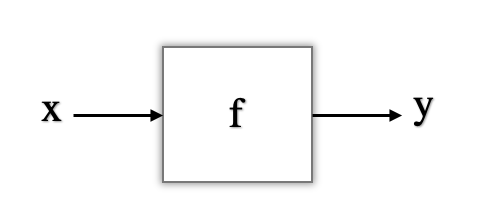
\includegraphics[width=0.5\linewidth]{figs/function_fx.png}
  \caption{Function f computing y on input x}
  \label{fig:fnxy}
  \end{figure} 
  
  \begin{figure}[h!]
  \centering
  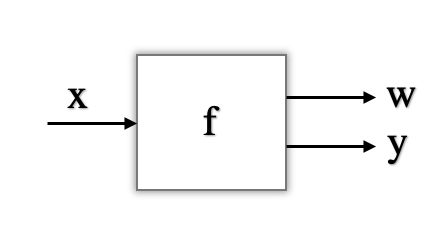
\includegraphics[width=0.5\linewidth]{figs/funcxy.png}
  \caption{Function f computing y and producing witness w on input x}
  \label{fig:fnxyw}
  \end{figure} 


%\begin{tikzpicture}
%\draw (0,0) rectangle (10,10) node[pos=0.5] {program for f};
%\end{tikzpicture}


  \noindent
   Below is a simple piece of Haskell code, but the choice of language does not matter as long as it 
   produces a certificate, which computes the greatest common divisor 
   of two numbers with a certificate (trace).  The first component of computation is the result and second one 
   the certificate. 
   \begin{verbatim}
   gcdWithCertificate :: Integer -> Integer -> (Integer, String)
   gcdWithCertificate a b
    | b == 0 = (a, "gcd " ++ show a ++ " 0 = " ++ show a)
    | otherwise = 
      let (rgcd, rcertificate) = gcdWithCertificate b (mod a b) in
      (rgcd, "gcd " ++ show a ++ " " ++ show b ++ "\n" ++ rcertificate)
   \end{verbatim}
  
   \noindent 
   After running the program on the concrete input 34 and 21, it produces the result and certificate (below).
   \begin{verbatim}
     gcd 34 21
     -------------
     gcd 21 13
     -------------
          .
     -------------
     gcd 1 0 
     -------------
        1
   \end{verbatim}
   
   
   In order to verify the correctness of the computation of greatest common divisor, we need to 
    make sure that one of the rules of Euclidean algorithm, given below, is applicable at 
    each line of the certificate:
   \begin{enumerate}
   \item Rule-zero: $\forall$ x, $\gcd$ x 0 = x
   \item Rule-inductive: $\forall$ x y, $\gcd$ x y = $\gcd$ y (mod x y)
   \end{enumerate}

 \noindent	
  The same certificate (augmented with rules and variables instantiated) from certificate-checker perspective.
    \begin{verbatim}
     gcd 34 21 = gcd 21 13 Rule-inductive: x := 34, y := 21, mod 34 21 = 13
     ---------------------------------------------------------------------
     gcd 21 13  = gcd 13 8 Rule-inductive: x := 21, y := 13, mod 21 13 = 8
     ---------------------------------------------------------------------
          .
     ---------------------------------------------------------------------
     gcd 1 0 = 1   Rule-zero: x := 0 
   \end{verbatim}
   
   
   Unfortunately, the example we gave,  greatest common divisor, is very simple, and 
   it is not 
   very helpful example to put the usefulness of certificate in perspective.
   However, this approach, generating a certificate to certify the computation later, is very useful in context 
   of complicated and unverified  programs.   One such example is algorithmic library  
   LEDA \citep{Mehlhorn:1995:LPC:204865.204889} ("Library of Efficient Data types and Algorithms") 
   written in C++.  Checkers are integral part of LEDA 
   which can later be invoked by user to certify that the result produced by unverified 
   code is correct. 
   Initially, the checkers came with library were unverified, and 
   Kurt Mehlhorn defended this decision by admitting that \citep{Alkassar2014}: 
   \begin{displayquote}
   Checkers are simple programs with little algorithmic 
   complexity. Hence, one may assume that their implementations are correct.
	\end{displayquote}   
	\noindent
    Later, the 
   checkers \citep{Alkassar2014} were verified by using VCC \citep{10.1007/978-3-642-03359-9_2}, 
   and Isabelle/Hol \citep{Nipkow:2002:IPA:1791547}.  One advantages of this approach is 
   that it is easier to formally verify the checker than the algorithm itself, because 
   checkers are very simple in nature, and this approach scales very well. 
   
   One may ask the question that can we follow the same approach for vote counting,
   i.e. unverified counting code, and verified checker?  The answer is: it depends. 
   If the verified checker validates the result, i.e. it returns true on  
   the certificate generated by unverified 
   vote counting program then everything is fine from every stakeholders' perspective.
   However, what about the situation when the verified checker returns false, i.e. invalidates 
   the result. This kind of situation must be dealt carefully by electoral commission, and commission should
   inspect everything carefully including the vote counting software and various other thing involved in the
   process.
   To eliminate this kind of problematic situation, we propose: i) a formally verified vote counting
   software which produces the result with evidence (certificate), and ii) formally verified 
   certificate checker. The advantage of this approach is that the result produced is always correct (modulo 
   specification), a confidence building measure for electoral commission. Furthermore, the verified checker would 
   always return true on the evidence (certificate) produced by verified vote counting program, confidence booster for 
   voters into the deployed system.  
  

%  We will discuss in more detail about certificate checking 
%  in chapter Software Independence.  We will also present a case study of 
%  formally verified checker for \textit{IACR 2018} (International Association for 
%  Cryptographic Research) election.
     
   
%  We have take 
%  
%  It is very crucial to know that the primary purpose of checkers are to verify the 
%  correctness of computation, hence, it is important that they 
%  should be: i) correct, and ii) simple.  
  
  
  
  
    
   
\section{Summary}
We reiterate that to maximise trust, reliability and auditability of electronic vote counting, we
need both approaches, verification and verifiability, to be combined. To ensure
verifiability, we advocate that vote-counting programs
do not only compute a final result, but additionally produce an
independently verifiable certificate that attests to the correctness
of the computation, together with a formal verification that
valid certificates indeed imply the correct determination of
winners. Given a certificate-producing vote-counting program, external
parties or stakeholders can then satisfy themselves to the
correctness of the count by checking the certificate.    

In the next chapter, I will  briefly discussion about Coq theorem prover and basic cryptographic primitives which 
would enable us later in counting encrypted ballots (without revealing any information about 
voter's choice).